\documentclass[graphics]{beamer}
\usepackage[utf8]{inputenc}
\usepackage[french]{babel}
\usepackage{lmodern}
\usepackage{tcolorbox}
\usepackage{pgfpages}
\usepackage{graphicx}
\usepackage{mathdots}
\usepackage{subcaption}
\usepackage{xcolor}
\usepackage[export]{adjustbox}
\usepackage{appendixnumberbeamer}
\usepackage{stmaryrd} 
\usepackage{caption}
\usepackage{version}
\usepackage{nicematrix}
\captionsetup[figure]{labelformat=empty}



\usetheme{Warsaw}
\usecolortheme{dolphin}

\title[Weak Schur numbers]{Weak Schur numbers}
\subtitle{P05 - Formation à la recherche}
\author[R. Ageron, P. Castéras, T. Pellerin, Y. Portella]{Romain Ageron, Paul Castéras, Thibaut Pellerin, Yann Portella}
\titlegraphic{\centering
	
\includegraphics[scale=.08]{cs}
}
%\institute[]{\'CentraleSupélec}
\date{1 février 2021}
	\setbeamersize{text margin left=15pt}
	\setbeamersize{text margin right=15pt}


% pour supprimer les symboles de navigation
\setbeamertemplate{navigation symbols}{}
% \setbeamertemplate{footline}[frame number]
\setbeamertemplate{caption}{\raggedright\insertcaption\par}

\newcommand\blfootnote[1]{%
	\begingroup
	\renewcommand\thefootnote{}\footnote{#1}%
	\addtocounter{footnote}{-1}%
	\endgroup
}

\begin{document}

\begin{frame}
\titlepage
%\begin{center}
%	\includegraphics[height=0.5cm]{logoens.pdf}
%\end{center}
\end{frame}

\section{Présentation}
\subsection{Un problème de partition}
\begin{frame}
	En 1917, le russe \textbf{Issai Schur} pose le problème suivant :
	\pause
	\begin{itemize}
		\item On se donne \(n \geq 1\) un entier
		\item \(k \geq 1\) un autre entier, qui correspond au nombre de \textbf{couleurs}
	\end{itemize}
	\pause
	\begin{tcolorbox}[colback=green!5,colframe=green!40!black,title=Question]
		Peut-on colorier les entiers de \(1\) à \(n\) de sorte que si deux nombres ont la même couleur,
		leur somme n'est pas de cette couleur ? Si oui, un tel coloriage est dit \textbf{sans sommes}.
	\end{tcolorbox}
\end{frame}

\subsection{Les nombres de Schur}

\begin{frame}
	Pour \(n = 13\) et \(k = 3\), le coloriage \\
	\begin{center}
	\begin{NiceTabular}{|*{13}{c|}}[standard-cline,hlines]
		\CodeBefore
			\cellcolor{red}{1-1}
			\cellcolor{blue}{1-2}
			\cellcolor{blue}{1-3}
			\cellcolor{red}{1-4}
			\cellcolor{green}{1-5}
			\cellcolor{green}{1-6}
			\cellcolor{blue}{1-7}
			\cellcolor{green}{1-8}
			\cellcolor{green}{1-9}
			\cellcolor{red}{1-10}
			\cellcolor{blue}{1-11}
			\cellcolor{blue}{1-12}
			\cellcolor{red}{1-13}
		\Body
			1 & 2 & 3 & 4 & 5 & 6 & 7 & 8 & 9 & 10 & 11 & 12 & 13\\
	\end{NiceTabular}
	\end{center}
	vérifie cette propriété.
	\pause
	\begin{tcolorbox}[colback=red!5,colframe=red!40!black,title=Définition]
		Pour \(k\) couleurs, on note \(S(k)\) le plus grand entier \(n\) tel qu'on puisse colorier les entiers de
		\(1\) à \(n\) en vérifiant cette propriété. C'est le \(k\)-ième \textbf{nombre de Schur}.
	\end{tcolorbox}
	\pause
	Sur l'exemple, on peut vérifier que \(S(3) = 13\) : on ne peut colorier \([\![1,14]\!]\) avec trois couleurs.
\end{frame}

\subsection{Weak Schur}

\begin{frame}
	\begin{tcolorbox}[colback=red!5,colframe=red!40!black,title=Définition]
		Un coloriage est dit \textbf{faiblement sans sommes} lorsque pour deux nombres \textbf{différents} de même couleur,
		leur somme n'est pas de la même couleur. On définit de même \(WS(k)\) le plus grand entier \(n\) tel qu'on puisse colorier les entiers de
		\(1\) à \(n\) en vérifiant cette propriété plus faible.
	\end{tcolorbox}
	\pause
	Un coloriage sans sommes et en particulier faiblement sans somme, donc on a toujours \(WS(k) \geq S(k)\).\\
	\pause 
	\begin{center}
	\begin{NiceTabular}{|*{4}{c|}}[standard-cline,hlines]
		\CodeBefore
			\cellcolor{red}{1-1}
			\cellcolor{blue}{1-2}
			\cellcolor{blue}{1-3}
			\cellcolor{red}{1-4}
		\Body
			1 & 2 & 3 & 4 \\
	\end{NiceTabular}

	\begin{NiceTabular}{|*{8}{c|}}[standard-cline,hlines]
		\CodeBefore
			\cellcolor{red}{1-1}
			\cellcolor{red}{1-2}
			\cellcolor{blue}{1-3}
			\cellcolor{red}{1-4}
			\cellcolor{blue}{1-5}
			\cellcolor{blue}{1-6}
			\cellcolor{blue}{1-7}
			\cellcolor{red}{1-8}
		\Body
			1 & 2 & 3 & 4 & 5 & 6 & 7 & 8 \\
	\end{NiceTabular}
	\end{center}
	\(S(2) = 4\) mais \(WS(2) = 8\)
\end{frame}

\section{L'état de l'art}
\subsection{Calculer ces nombres}

\begin{frame}
	\begin{itemize}
	\item Pour montrer que \(S(k) = n\), il faut trouver un coloriage sans sommes de \([\![1,n]\!]\) à \(k\) couleurs
	\textbf{et} montrer qu'on ne peut pas colorier \([\![1,n+1]\!]\). 
	\pause
	\item En pratique, on se contente de \textbf{minorer} \(S(k\). Si on exhibe un coloriage à \(k\) couleurs de 
	\([\![1,n]\!]\), on a montré que \(S(k) \geq n\). 
	\pause
	\item Comment effectuer cette minoration ? On peut démontrer des inégalités récursives ou bien rechercher des coloriages
	par ordinateur.
	\end{itemize}
\end{frame}

\subsection{Approche numérique}

\begin{frame}
	Les recherches récentes sur le sujet se focalisent sur les méthodes numériques.
	\begin{itemize}
		\item On fixe \(k\) et on essaye de colorier le plus loin possible
		\item Le problème peut s'encoder comme une exploration d'arbre, mais le nombre de coloriages possibles
		explose très vite 
		\item Plusieurs articles récents ont recourt à l'algorithme \textbf{Monte-Carlo Tree Search}, et ne considèrent 
		que certains type de coloriages
		\item On peut également encoder le problème avec un solveur \textbf{SAT} 
	\end{itemize}
	\pause
	Ces méthodes ont permis d'améliorer les bornes inférieures pour \(k \geq 5\) mais peuvent prendre du temps :
	récemment, le calcul exact de \(S(5)\) via un solveur SAT a demandé 20 années de calcul machine.
\end{frame}

\section{Découpage du code}

\subsection{Méthode d'évaluation}

\begin{frame}
	\begin{figure}[H]
		\centering
		\begin{subfigure}[b]{0.4\textwidth}
			\centering
			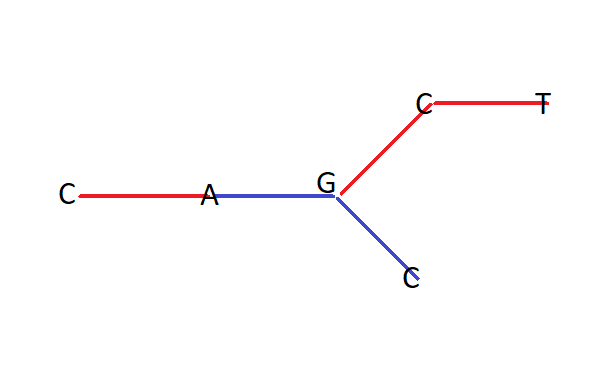
\includegraphics[width=\textwidth]{pb_angle}
			\caption{Bonne distance mais mauvaise orientation}
			\label{fig:y equals x}
		\end{subfigure}
		\begin{subfigure}[b]{0.4\textwidth}
			\centering
			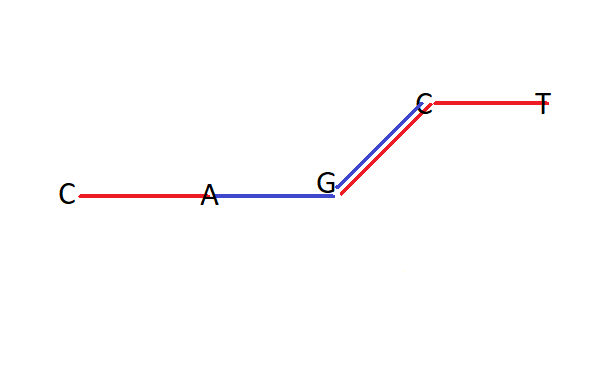
\includegraphics[width=\textwidth]{angle_oui}
			\caption{Bonne distance et bonne orientation}
			\label{fig:three sin x}
		\end{subfigure}
		\caption{Jonction pour une chaîne $GCT...CA$}
		\label{fig:three graphs}
	\end{figure}
Pour contrôler la qualité de la trajectoire, on ajoute (en bleu) les deux premiers nucléotides à la fin de la chaîne. Ici, $G$, le premier nucléotide, est bien placé mais l'orientation de $GC$ n'est pas forcément valide.
\end{frame}

\subsection{Classes} 





\begin{frame}
	L'étape de mutation s'est révélée très importante :
	\begin{itemize}
		\item elle permet d'explorer l'espace du problème 
		\item des mutations trop limitées bloquent l'algorithme dans des minimums locaux
		\item des mutations excessives risquent de gâcher des individus prometteurs
	\end{itemize}
Nous avons choisi de faire muter une part importante de la population, mais pas les individus ayant les meilleurs scores. La mutation modifie une des variables, aléatoirement dans l'intervalle associé.
\end{frame}

\section{Résultats}
\subsection{Quelques images}

\begin{frame}
	La trajectoire totale est représentée à gauche, et la jonction à droite (un vecteur = un dinucléotide).
	\begin{figure}[H]
		\centering
		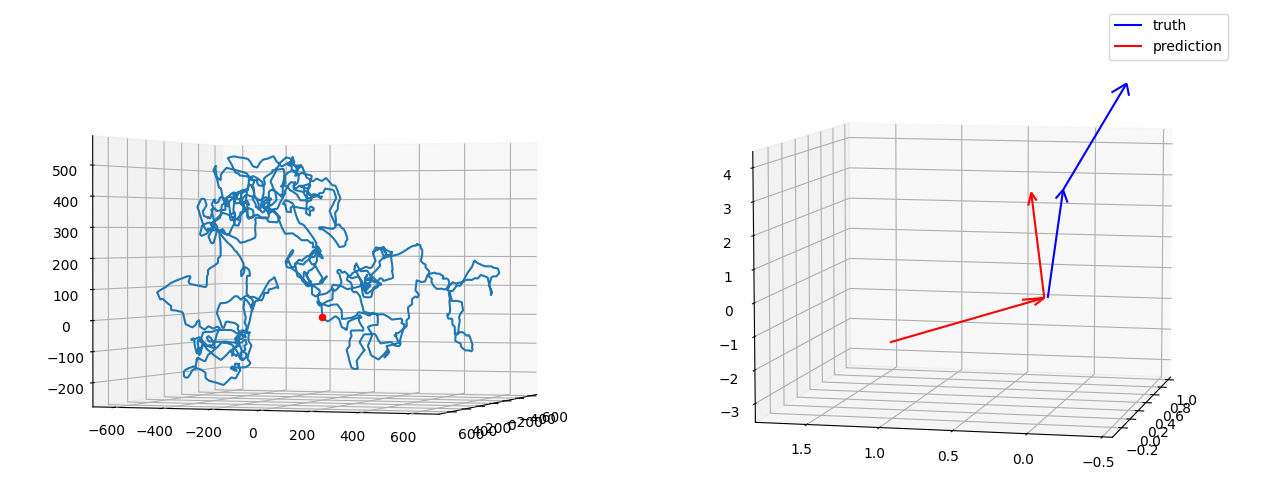
\includegraphics[scale=0.3]{8k_200gen_1000pop_tour0.3_mut0.7_1.038}
		\caption{Une chaîne de longueur 8000, avec 200 générations et une population de 1000}
	\end{figure}
	Ici, l'erreur de position est faible mais celle d'orientation non négligeable.
\end{frame}

\begin{frame}
	On peut modifier légèrement la fonction  afin de pénaliser davantage l'erreur sur l'angle.
	\begin{figure}[H]
		\centering
		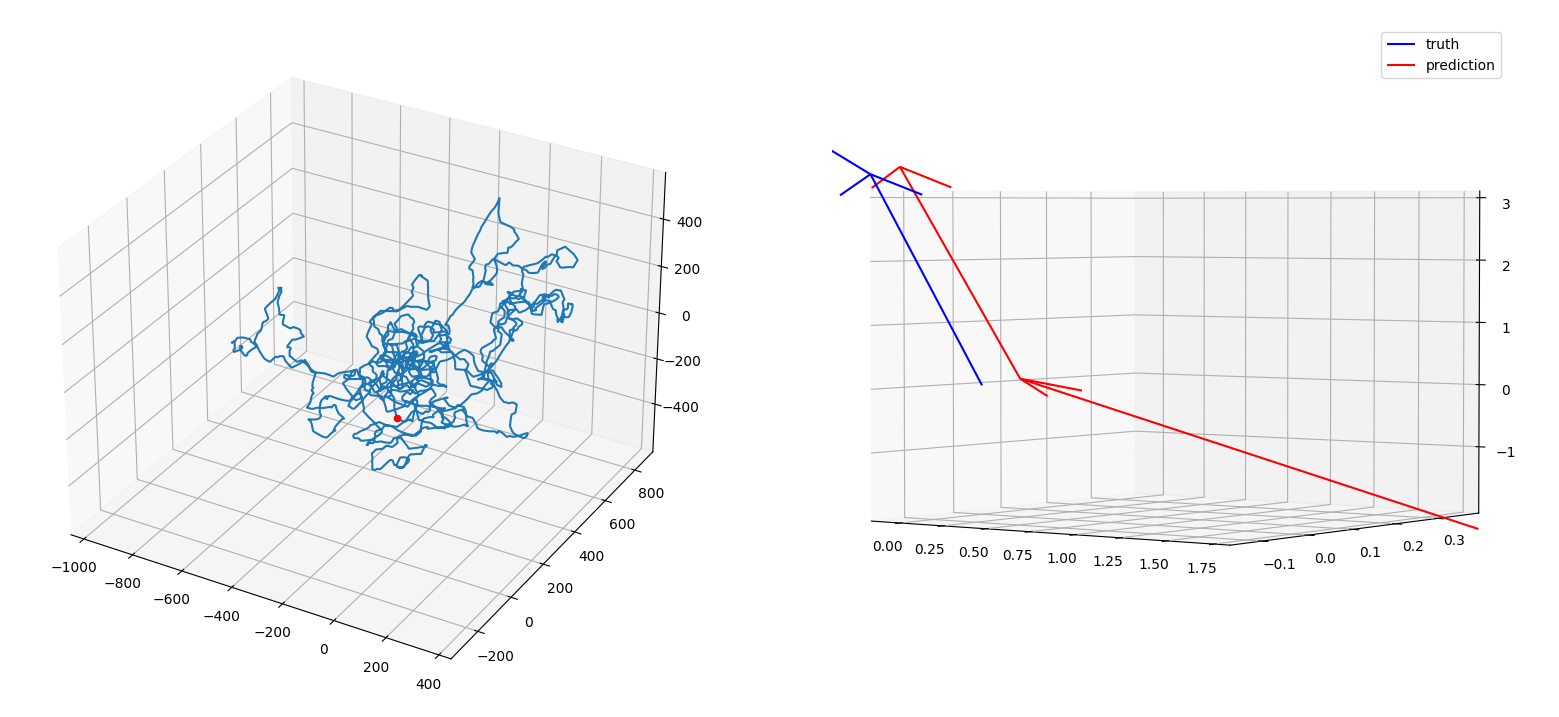
\includegraphics[scale=0.25]{250gen200pop0.3_0.003_0.7_0.003alpha=10}
		\caption{Une chaîne de longueur 8000, avec 250 générations et une population de 200}
	\end{figure}
	Les dinucléotides réel et fictif sont ici parallèles, mais la distance est plus importante.
\end{frame}

\begin{frame}
	Après une bonne heure de calcul, on obtient ceci pour une chaîne de 180000 nucléotides.
	\begin{figure}[H]
		\centering
		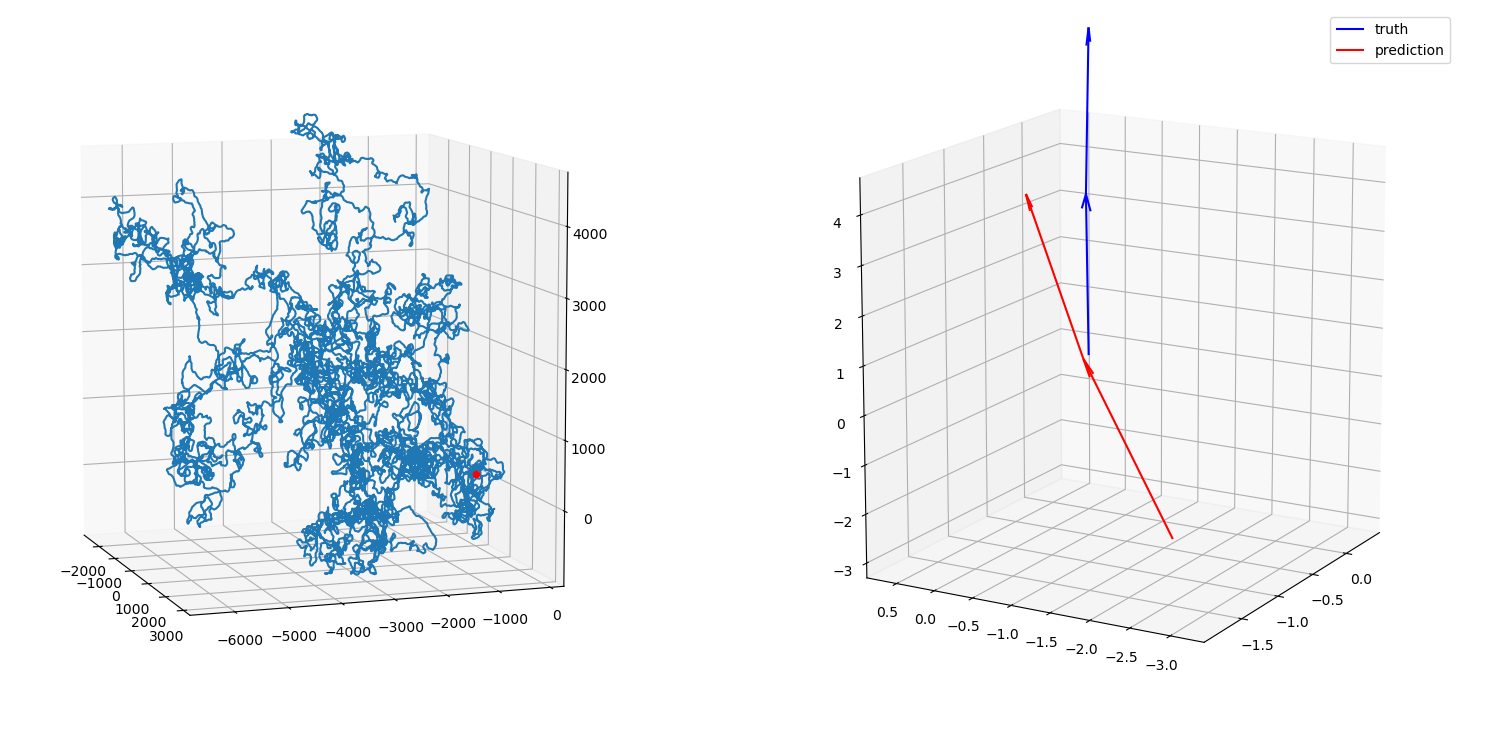
\includegraphics[scale=0.25]{180}
	\end{figure}
\end{frame}

\subsection{Commentaires}
	
\begin{frame}
	\begin{itemize}
		\item Le temps d'exécution est d'environ 3 minutes pour une chaîne de longueur 8000, une population de 100 et une centaine de générations
		\item L'accumulation d'erreurs numériques rend les résultats pour la chaîne de 180k peu fiables
		\item Difficile d'équilibrer la fonction  afin d'avoir une bonne distance et une bonne orientation
	\end{itemize}
\end{frame}

\subsection{Ouverture}

\begin{frame}
Ici, l'optimisation est \textbf{multi-critère}. Nous nous sommes ramené à une fonction  scalaire, mais il peut être plus efficace de mesurer indépendamment les deux erreurs. \\
On se prive alors de l'ordre sur $\mathbb{R}$, mais on peut pallier ce problème en utilisant par exemple des \textit{fronts de Pareto}.
\begin{figure}[H]
	\centering
	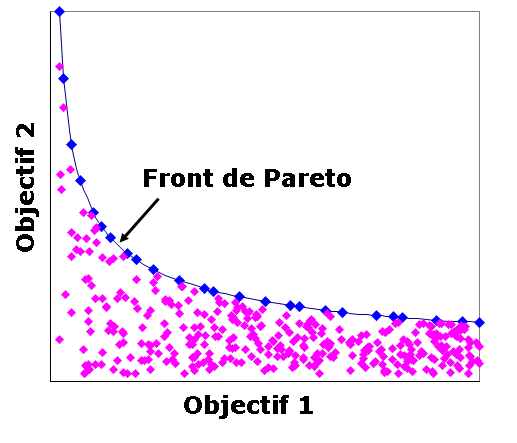
\includegraphics[scale=0.3]{pareto}
\end{figure}

Une autre idée serait de faire une fonction de mutation dynamique (par exemple plus de mutation lorsque l'algorithme stagne).
\end{frame}

\end{document}